\subsection{Mutacja}

Zadaniem mutacji jest wprowadzenie różnorodności w populacji. Dlatego we własnej implementacji zostały wprowadzone elementy losowości.

\subsubsection{Kod źródłowy}

\begin{lstlisting}[linewidth=16.0cm]
myMutation <- function (ga_object, parent) 
{
  # Pobranie osobnikow do mutacji
  mutate <- parent <- as.vector(ga_object@population[parent,])
  parLen <- length(parent)
  
  all <- c(1:parLen)
  # Wykluczenie losowych osobnikow z mutacji
  excluded <- sample(1:parLen/4, size = 1)
  indexesToMutate <- all[!excluded]
  
  # Mutacja przy uzyciu losowych wartosci
  mutate[indexesToMutate] <- mutate[indexesToMutate] - rnorm(n=1, m=0, sd=3)

  return(mutate)
} 
\end{lstlisting}

\subsubsection{Wyniki badań}

\begin{figure}[H]
	\centering
	\hspace*{-0.8in}
	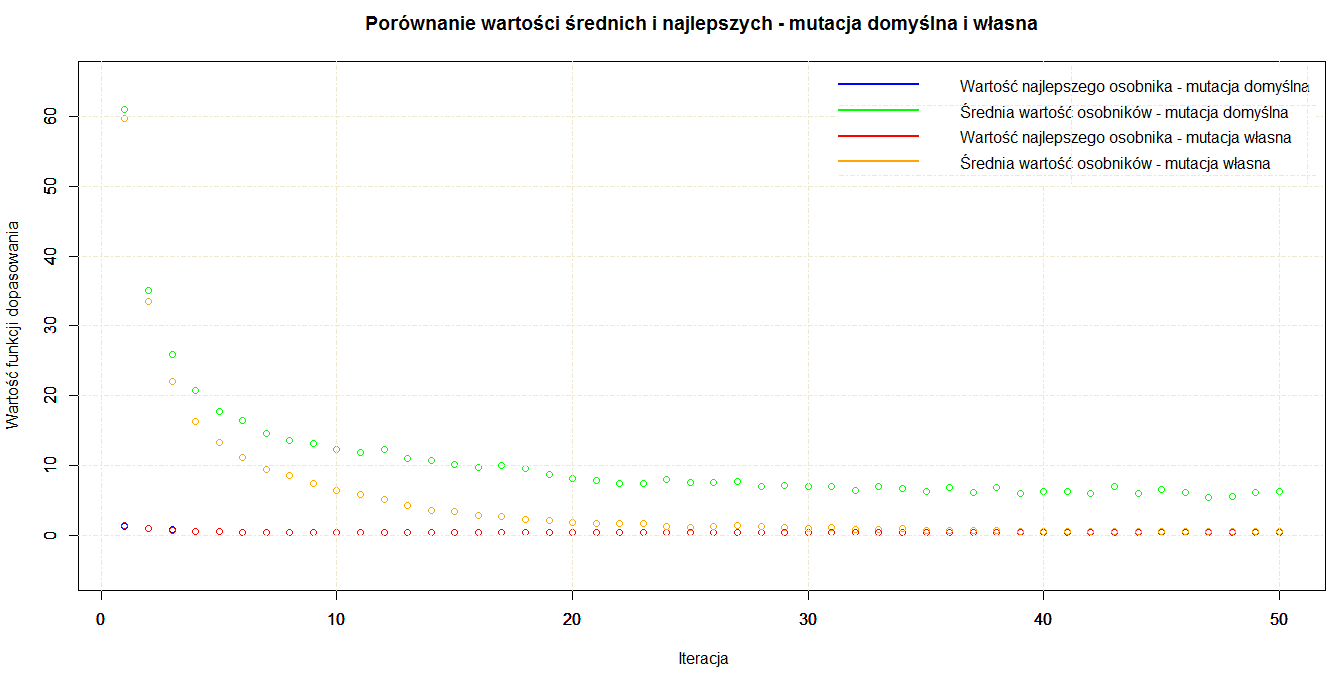
\includegraphics[scale = 0.5]{img/zad1/mut_0_1}
	\caption{Wykres dla prawdopodobieństwa mutacji 0.1}  
	\label{rys:mut_0.1} 
\end{figure}

\begin{figure}[H]
	\centering
	\hspace*{-0.8in}
	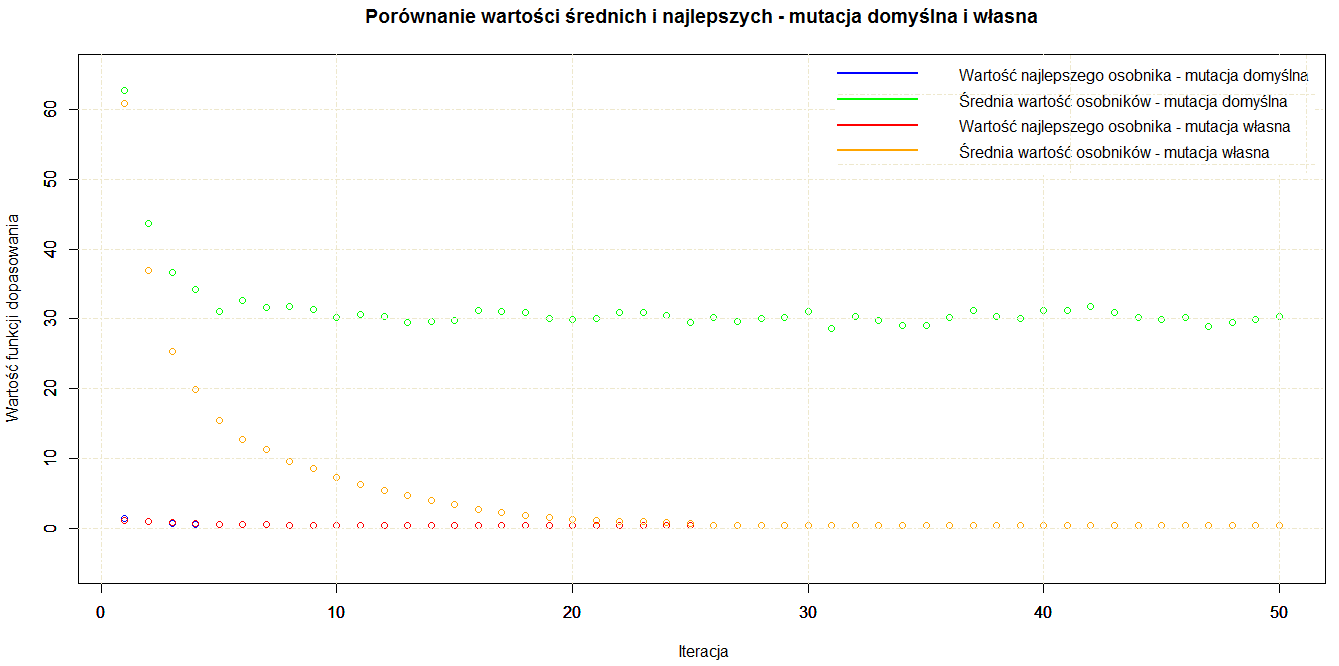
\includegraphics[scale = 0.5]{img/zad1/mut_0_5}
	\caption{Wykres dla prawdopodobieństwa mutacji 0.5}  
	\label{rys:mut_0.5} 
\end{figure}

\begin{figure}[H]
	\centering
	\hspace*{-0.8in}
	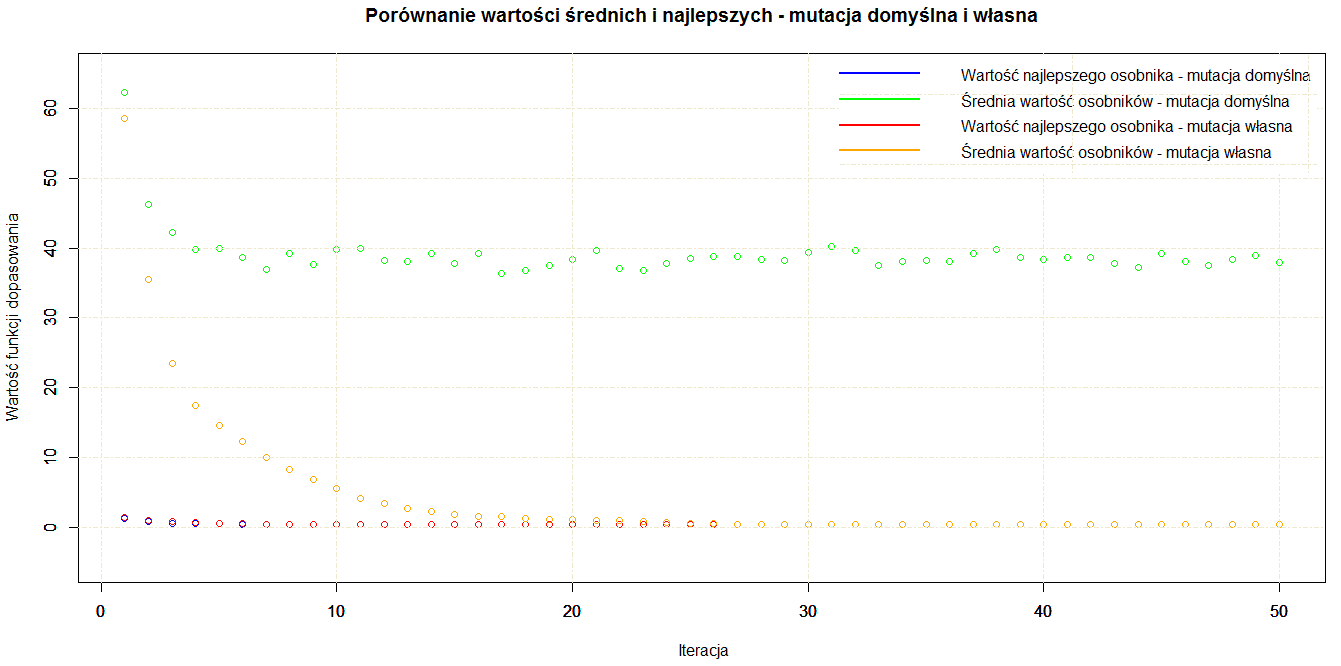
\includegraphics[scale = 0.5]{img/zad1/mut_0_7}
	\caption{Wykres dla prawdopodobieństwa mutacji 0.7}  
	\label{rys:mut_0.7} 
\end{figure}

\begin{figure}[H]
	\centering
	\hspace*{-0.8in}
	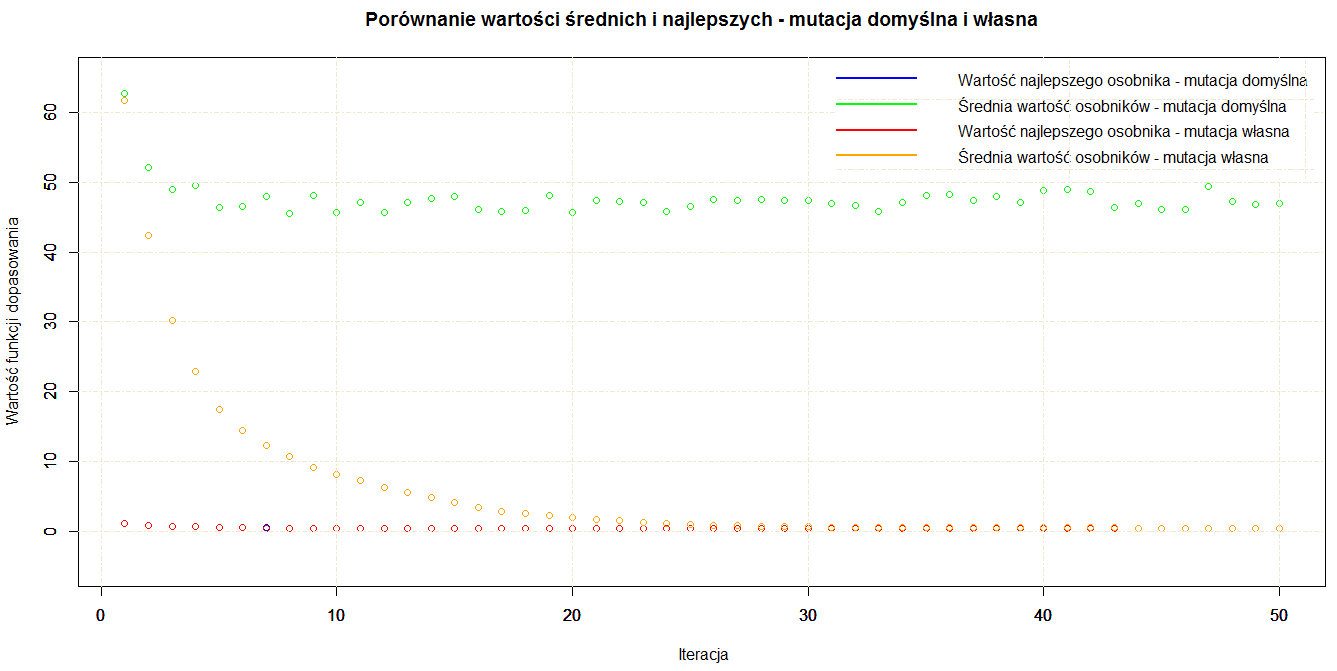
\includegraphics[scale = 0.5]{img/zad1/mut_1}
	\caption{Wykres dla prawdopodobieństwa mutacji 1}  
	\label{rys:mut_1} 
\end{figure}

\vline

\subsubsection{Wnioski}

\begin{table}[!h]
	\hspace*{-1.5in}
	\centering
	\caption{Wartości średnie i najlepsze osobnika dla domyślnej i własnej funkcji mutacji}
	\label{mut_porownanie}
	\hspace*{-0.4in}
	\begin{tabular}{|c|c|c|c|c|}
		\hline
		\textbf{Prawdopodobieństwo} & \multicolumn{2}{c}{\textbf{Mutacja domyślna}}  & \multicolumn{2}{|c|}{\textbf{Mutacja własna}} \\ \cline{2-5}
		\textbf{mutacji} & Wartość średnia & Najlepszy wynik & Wartość średnia & Najlepszy wynik \\ \hline
		
		0.1 & 5.753710  & \textbf{{\color{green} 0.398006 }} & 0.398736 & 0.398687 \\
		0.5 & 31.029570 & 0.401904 & 0.415733 & 0.398201 \\
		0.7 & 38.184020 & 0.404532 & 0.567679 & 0.398926 \\
		1   & 46.920430 & 0.408154 & 0.452637 & 0.400847  \\ \hline      
	\end{tabular}
\end{table}

Na wykresach można łatwo zauważyć, że wybór funkcji mutacji nie wpłynął znacząco na wartości najlepszego osobnika w populacji, natomiast wartości średnie wyraźnie odstają od siebie dla tych dwóch przypadków. Można stąd wywnioskować, że własna implementacja mutacji wykonuje mniej inwazyjne operacje na osobnikach. \\
Natomiast najlepszy wynik przy tej ilości iteracji został osiągnięty podczas uruchomienia algorytmu z ustawieniami domyślnymi. Implementacja mutacji nie poprawiła więc wyników działania algorytmu.